\documentclass[../assignment2.tex]{subfiles}
\graphicspath{{\subfix{../figures/assignment2/}}}

\begin{document}
\begin{figure}[h]
    \centering
    \subcaptionbox{Inverse Fourier transform of sampling function \label{frequency-sampling}}{
        \resizebox{0.45\textwidth}{!}{
            \begin{tikzpicture}
            % \draw[help lines, color=gray!30, dashed] (-3.9,-3.9) grid (3.9,3.9);
            \draw[->,ultra thick] (-4,0)--(4,0) node[right]{$x$};
            \draw[->,ultra thick] (0,-4)--(0,4) node[above]{$y$};
            
            \foreach\x/\label in {-3/$-2\pi$, -1.5/$-\pi$, 0/$0$, 1.5/$\pi$, 3/$2\pi$}
                \filldraw[red] (\x,0) circle (2pt) node[below,black]{\label};
            
            \foreach\y/\label in {-3/$-2\pi$, -1.5/$-\pi$, 1.5/$\pi$, 3/$2\pi$}
                \filldraw[red] (0,\y) circle (2pt) node[left,black]{\label};
            
            \foreach \x in {-3, -1.5, 1.5, 3}
                \foreach \y in {-3, -1.5, 1.5, 3}
                    \filldraw[red] (\x,\y) circle (2pt) node{};
            \end{tikzpicture}
        }
    }
    \hfill
    \subcaptionbox{Aliasing-free frequency interval \label{frequency-sampling-2}}{
        \resizebox{0.45\textwidth}{!}{
            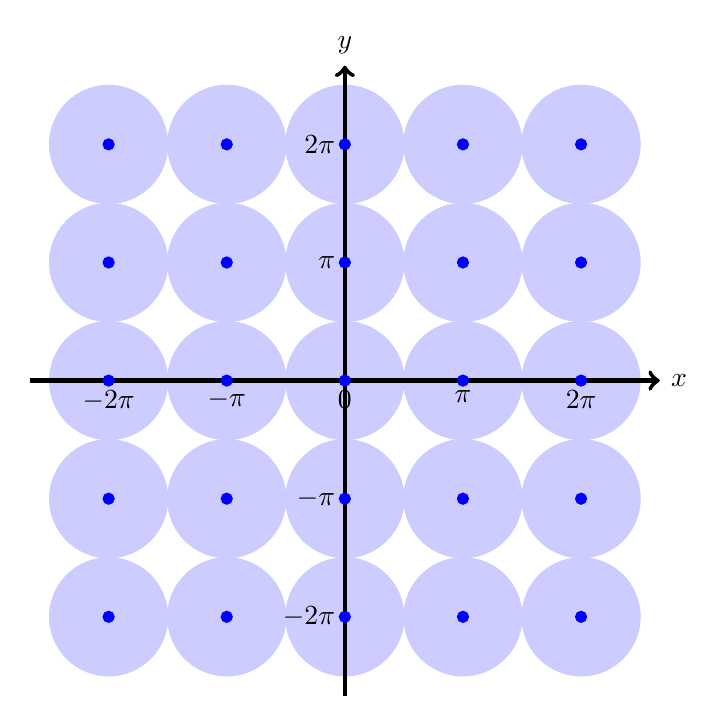
\begin{tikzpicture}
            % \draw[help lines, color=gray!30, dashed] (-3.9,-3.9) grid (3.9,3.9);
            \foreach \x in {-3, -1.5, 0, 1.5, 3}
                \foreach \y in {-3, -1.5, 0, 1.5, 3}
                    \filldraw[blue!20] (\x,\y) circle (0.75cm) node{};
                    
            \draw[->,ultra thick] (-4,0)--(4,0) node[right]{$x$};
            \draw[->,ultra thick] (0,-4)--(0,4) node[above]{$y$};

            \foreach\x/\label in {-3/$-2\pi$, -1.5/$-\pi$, 0/$0$, 1.5/$\pi$, 3/$2\pi$}
                \filldraw[blue] (\x,0) circle (2pt) node[below,black]{\label};
            
            \foreach\y/\label in {-3/$-2\pi$, -1.5/$-\pi$, 1.5/$\pi$, 3/$2\pi$}
                \filldraw[blue] (0,\y) circle (2pt) node[left,black]{\label};
            
            \foreach \x in {-3, -1.5, 1.5, 3}
                \foreach \y in {-3, -1.5, 1.5, 3}
                    \filldraw[blue] (\x,\y) circle (2pt) node{};
            \end{tikzpicture}
        }
    }
    \caption{Frequency domain (2D)}
\end{figure}
\end{document}

\centering
    \subcaptionbox{x \label{}}{
        \resizebox{0.45\textwidth}{!}{
            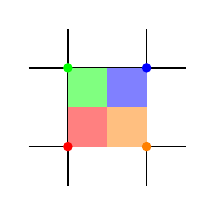
\begin{tikzpicture}
                \draw[step=1cm,black,semithick] (0.5,0.5) grid (2.5,2.5);
                \fill[red!50] (1,1) rectangle (1.5,1.5);
                \fill[green!50] (1,1.5) rectangle (1.5,2);
                \fill[orange!50] (1.5,1) rectangle (2,1.5);
                \fill[blue!50] (1.5,1.5) rectangle (2,2);
                \filldraw[red] (1,1) circle (1.5pt) node {};
                \filldraw[green] (1,2) circle (1.5pt) node {};
                \filldraw[orange] (2,1) circle (1.5pt) node {};
                \filldraw[blue] (2,2) circle (1.5pt) node {};
            \end{tikzpicture}
        }
    }
    \hfill